%26
\begin{frame}
  Szövegrészek idézése. Forrás jelölése: \texttt{cite} attribútummal.
  \begin{description}[m]
    \item[\texttt{<q>}] (quote) \hfill \\ Rövid szövegrészlet idézése, ált. automatikusan körbeveszi a böngésző idézőjelekkel. Soron belüli elem.
    \item[\texttt{<blockquote>}] \hfill \\ Hosszú szövegrészek, bekezdések idézése. Jellemzően behúzással formázva. Blokkszintű elem.
  \end{description}
  \vfill
  Rövidítések. Kifejtés megadható: \texttt{title} globális attribútummal.
  \begin{description}[m]
    \item[\texttt{<abbr>}] \hfill \\ Rövidítések és betűszavak jelöléséhez. Soron belüli elem.
    \item[\texttt{<acronym>}] \hfill \\ Betűszavak jelöléséhez használták, \kiemel{ELAVULT}.
  \end{description}
\end{frame}

%27
\begin{frame}
  Szöveg írásirányának jelölése: \texttt{dir} globális attribútummal, alapértelmezést a nyelvvel együtt a \texttt{html} elemben kell állítani. Értékek:
  \begin{description}[m]
    \item[\texttt{ltr}] (left to right) \hfill \\ balról jobbra
    \item[\texttt{rtl}] (right to left) \hfill \\ jobbról balra
  \end{description}
  \vfill
  Írásirány helyi módosítása: \texttt{<bdo>} (Bi-Directional Override) elemmel, \texttt{dir} attribútummal
  \vfill
  Mű címének jelölése: \texttt{<cite>} soron belüli elemmel.
  \vfill
  Postacím megadása: \texttt{<address>} blokkszintű elemmel.
\end{frame}

%28
\begin{frame}
  \begin{columns}[c]
    \column{0.6\textwidth}
      Próbálja meg előállítani azt a HTML fájlt, ami a jobb oldalon látható módon jelenik meg a böngészőben!
      Kiinduláshoz felhasználhatja a dokumentum \textattachfile{idezes.txt}{nyers szövegét}.
      Az idézőjelek többféle szélességben elérhetők: \texttt{\&ndash;}, \texttt{\&mdash;}.
    \column{0.4\textwidth}
      \begin{center}
        \begin{exampleblock}{\textattachfile{idezes.html}{idezes.html}}
          \centering 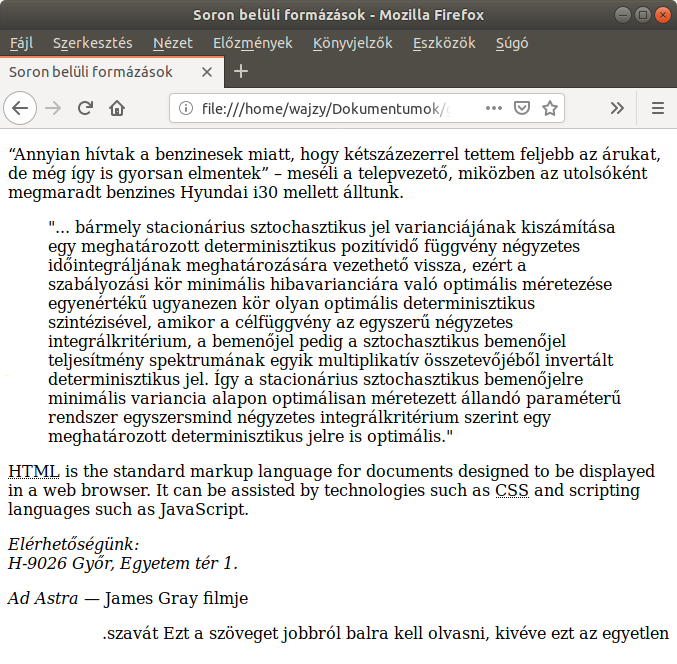
\includegraphics[scale=.23]{idezes.png}
        \end{exampleblock}
      \end{center}
  \end{columns}
\end{frame}
